\section{Microlenses}
\label{sec:microlenses}

This section is devoted to exploring the phenomenon of microlensing, which refers to the lensing effects caused by objects of relatively small mass in the universe, such as planets, stars, star clusters, and other compact objects located within the Milky Way or distant galaxies. Typically, these microlenses are considered, in a first-order approximation, to be point-masses or collections of point-masses.


%%%%%%%%%%%%%%%%%%%%%%%%%%%%%%%%%%%%%%%%%%%%%%%%%%%%%%%
%%%%% Deflection angle and lensing potential %%%%%
%%%%%%%%%%%%%%%%%%%%%%%%%%%%%%%%%%%%%%%%%%%%%%%%%%%%%%%
\subsection{Deflection angle and lensing potential}
\label{subsec:angle_potential}
As already derived with \cref{eq:2.5}, by setting the lens position as the center of the reference frame and using the relation $\x = D_L \t$, the deflection angle for a point mass lens can be written as
\be
\label{eq:3.1}
\va{\a} (\va{\t}) = \frac{D_{LS}}{D_S} \hat{\va{\a}} (\va{\t}) = \frac{D_{LS}}{D_S} \frac{4 G M}{c^2 D_L} \frac{\va{\t}}{|\va{\t}|^2} \,.
\ee

Given that $\va{\a} (\va{\t}) = \va{\nabla} \hat{\P} (\va{\t})$, the lensing potential of the point mass lens is
\be
\label{eq:3.2}
\hat{\P} (\va{\t}) = \frac{4 G M}{c^2} \frac{D_{LS}}{D_L D_S} \ln{|\va{\t}|} \,.
\ee


%%%%%%%%%%%%%%%%%%%%%%%%%%%%%%%%%%%%%%%%%%%%%%%%%%%%%%%
%%%%% Lens equation and multiple images %%%%%
%%%%%%%%%%%%%%%%%%%%%%%%%%%%%%%%%%%%%%%%%%%%%%%%%%%%%%%
\subsection{Lens equation and multiple images}
\label{subsec:lenseq_images}
Given the deflection angle of \cref{eq:3.1}, the lens equation becomes
\be
\label{eq:3.3}
\b = \t - \frac{4 G M}{c^2 \t} \frac{D_{LS}}{D_L D_S} \,,
\ee
where the vector signs can be omitted due to the fact that the vector $\hat{\va{\a}}$ always points away from the lens.

As already anticipated in \cref{sec:lens_equation}, the lens equation can be written in a more concise way by introducing a scale radius $\t_E$, \ie the \emph{Einstein radius} defined in \cref{eq:2.30}, and setting $y = \b / \t_E$ and $x = \t / \t_E$, results:
\be
\label{eq:3.4}
\b = \t - \frac{\t_E^2}{\t} \quad \Rightarrow \quad y = x - \frac{1}{x} \,.
\ee
This equation is quadratic in $\t$ (or $x$) and has two solutions:
\be
\label{eq:3.5}
x_\pm = \frac{y \pm \sqrt{y^2 + 4}}{2} \,,
\ee
which means that there always exist two images for a given source position.

\begin{figure}
    \centering
    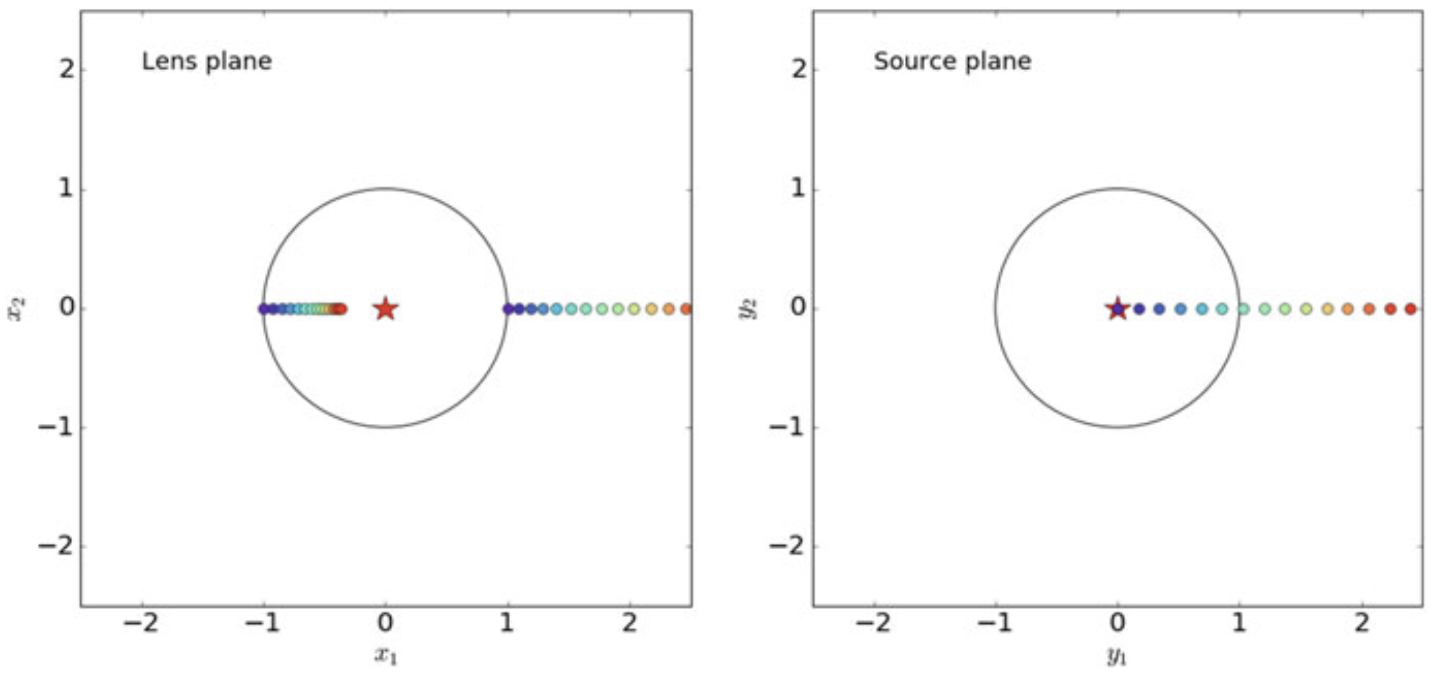
\includegraphics[width=\linewidth, keepaspectratio]{img//chapter3/pointmass_solutions.png}
    \caption[Lens equation solutions for point-mass lens]{Solutions of the lens equation for a point-mass, with the lens represented by the star at the center. The Einstein ring is highlighted in black. In the right diagram, the locations of various sources are marked with colored circles. The images produced, as calculated using \cref{eq:3.5}, are displayed in the left diagram.\\\small{Credits: \cite{meneghetti_introduction_2021}.}}
    \label{fig:pointmass_solutions}
\end{figure}

In the right section of \cref{fig:pointmass_solutions}, some sources are arranged at varying angular distances from the lens, which is marked by a red star. Each source is represented by a unique color to facilitate the identification of its corresponding images in the left section. Each source generates two images: one positioned at $x_+ > 0$ and the other in the range of $-1 < x_- < 0$. These images appear on either side of the lens, with the $x_-$ image always lying within a circle of radius $x = 1$. This circle is equivalent to the image produced by a source directly behind the point lens at $y = 0$, resulting in a ring-shaped image with radius $\t_E$, the Einstein ring.
The size of the Einstein radius is typically
\be
\label{eq:3.6}
\t_E \approx \SI{1}{\arcsecond} \bp{\frac{M}{10^{12} M_\odot}}^{1/2} \bp{\frac{D}{\si{\giga\parsec}}}^{-1/2} \,,
\ee
where
\be
\label{eq:3.7}
D \equiv \dfrac{D_L D_S}{D_{LS}}
\ee
is the \emph{effective lensing distance}.

As the angular separation $y \rightarrow 0$, it is observed that $x_- \rightarrow 0$, whereas $x_+ \rightarrow y$. This indicates that when the angular distance between the lens and the source increases significantly, the source is unlensed. In theory, an image still exists at $x_- = 0$, but this central image has zero magnification.


%%%%%%%%%%%%%%%%%%%%%%%%%%%%%%%%%%%%%%%%%%%%%%%%%%%%%%%
%%%%% Critical lines, caustics and magnification %%%%%
%%%%%%%%%%%%%%%%%%%%%%%%%%%%%%%%%%%%%%%%%%%%%%%%%%%%%%%
\subsection{Critical lines, caustics and magnification}
\label{subsec:critlines_caustics}
The Jacobian determinant for a point-mass lens can be written as
\be
\label{eq:3.8}
\det A (x) = \frac{y}{x} \frac{\dd{y}}{\dd{x}} \,,
\ee
which means that the eigenvalues of the Jacobian matrix are
\begin{subequations}
\begin{align}
    \label{eq:3.9a}
    \l_t (x) & = \frac{y}{x} = \bp{1 - \frac{1}{x^2}} \,,
    \\
    \label{eq:3.9b}
    \l_r (x) & = \frac{\dd{y}}{\dd{x}} = \bp{1 + \frac{1}{x^2}} \,.
\end{align}
\end{subequations}

The second eigenvalue is never zero, and therefore the point-mass lens only has a tangential critical line, a circle with equation $x^2 = 1$, which represents the Einstein ring.
This line can be mapped onto the source plane to find the relative tangential caustic, resulting in a single point at $y = 0$.

Given that the magnification is the inverse of the Jacobian determinant
\be
\label{eq:3.10}
\m (x) = \bp{1 - \frac{1}{x^4}}^{-1} \,,
\ee
which can also be written as a function of the source position
\be
\label{eq:3.11}
\m_\pm (y) = \frac{x}{y} \frac{\dd{x}}{\dd{y}} = \frac{1}{2} \bp{1 \pm \frac{y^2 + 2}{y \sqrt{y^2 + 4}}} \,,
\ee
the magnifications of the two images always have the same signs of $x_\pm$ and therefore different parity.

The total source magnification will then be:
\be
\label{eq:3.12}
\m (y) = \m_+ (y)  + |\m_- (y)| = \frac{y^2 + 2}{y \sqrt{y^2 + 4}} \,,
\ee
while the sum of the signed magnifications is always $\m = 1$.

Furthermore, it can be shown through series expansion that, for large $y$,
\be
\label{eq:3.13}
\lim_{y\to\infty} \left| \frac{\m_+}{\m_-} \right| \propto y^4 \,.
\ee
This means that the magnification rapidly becomes negligible outside the Einstein ring and has a very simple form well inside it. Hence, deviations from simple point-lens microlensing can usually be easily spotted.


%%%%%%%%%%%%%%%%%%%%%%%%%%%%%%%%%%%%%%%%%%%%%%%%%%%%%%%
%%%%% Microlensing light-curve %%%%%
%%%%%%%%%%%%%%%%%%%%%%%%%%%%%%%%%%%%%%%%%%%%%%%%%%%%%%%
\subsection{Microlensing light-curve}
\label{subsec:micro_lc}
The Einstein radius of a typical lens indicates the scale of image separation observed in microlensing events. For a star with the mass of the Sun located within the Milky Way, the separation is approximately of the order of milliarcseconds, a measurement that is beyond the detection capabilities of current instruments. However, stars move around the Galactic center (and have an additional random velocity component with respect to one another). The relative velocities are such that the time scale of the relative change of lens and source positions is of order of weeks or shorter. Therefore, this motion introduces a temporal component in the lensing geometry, causing the distance between the lens and the source, and thus the magnification, to vary measurably as a function of time, accordingly to \cref{eq:3.12}. In general, a source with intrinsic flux $F_s$ will appear to have flux $F (t) = \m (t) F_s$. 
\newpage
The \emph{microlensing light-curve} describes the temporal behavior of the magnification, dictated by the relative motion of the lens across the observer-source line of sight.

\begin{figure}
    \centering
    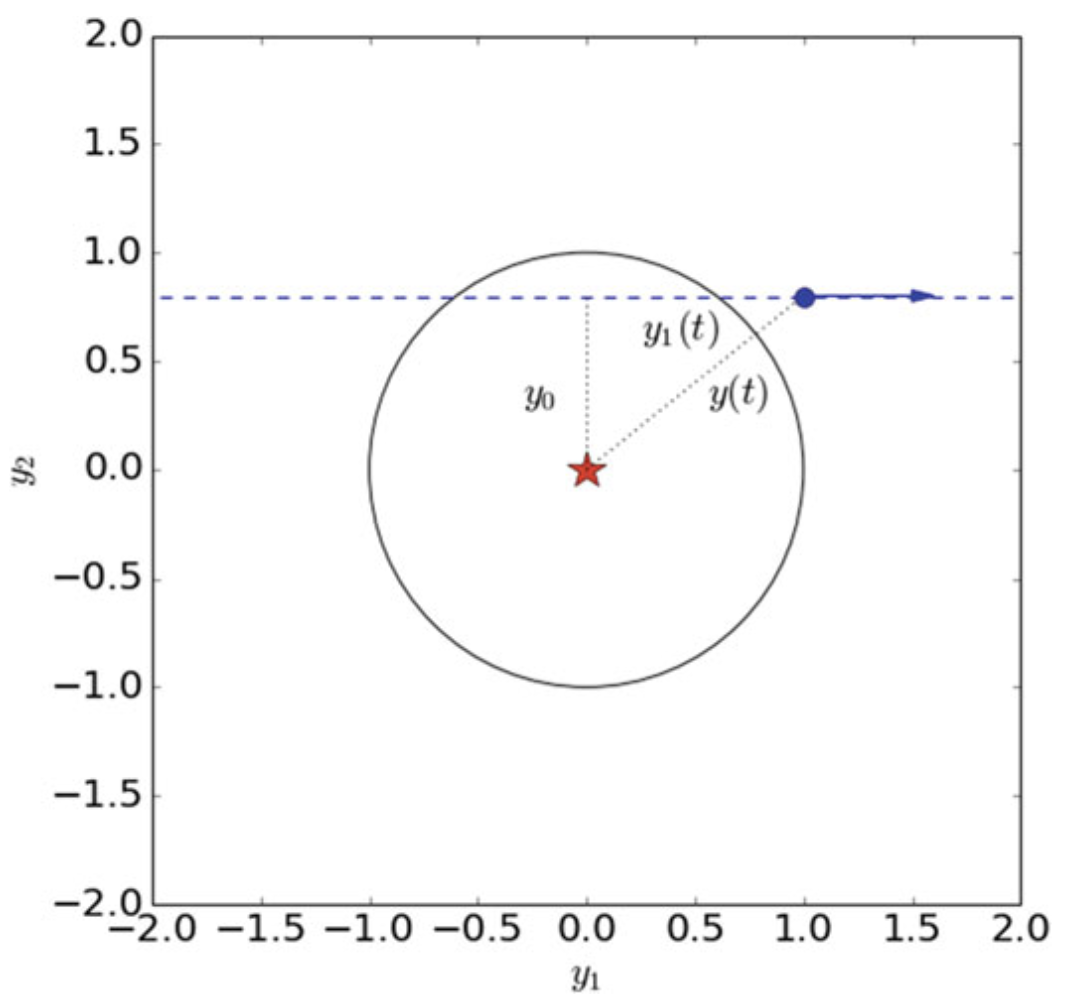
\includegraphics[width=0.61\linewidth, keepaspectratio]{img//chapter3/lens_source_trajectory.png}
    \caption[Lens position and source trajectory in a microlensing event]{Illustration of the lens position and source trajectory. The dimensionless impact parameter is $y_0$, $y_1 (t)$ indicates the dimensionless distance of the source from its closest point to the lens, and $y (t)$ is the dimensionless distance between the lens and source.\\\small{Credits: \cite{meneghetti_introduction_2021}.}}
    \label{fig:lens_source_trajectory}
\end{figure}

As shown in \cref{fig:lens_source_trajectory}, assuming a straight line can approximate the path of the source relative to the lens, the former moving with transverse velocity $v$ and reaching the minimum dimensionless distance $y_0$ (\ie the \emph{impact parameter} of the source), from the lens at time $t_0$, the dimensionless distance of the source from $y_0$ can be written
\be
\label{eq:3.14}
y_1 (t) = \frac{v (t - t_0)}{D_L \t_E} \,.
\ee

Since magnification significantly deviates from unity only for sources with $|y| \lesssim 1$, the characteristic timescale of the microlensing event is given by
\be
\label{eq:3.15}
t_E = \frac{D_L \t_E}{v} \,,
\ee
which is known as the \emph{Einstein crossing time}. Stellar lenses in the Milky Way are associated with typical $t_E$ on the order of a month, and thus the changes in the observed brightness of the source they induce are referred to as microlensing ``events''.

Inserting \cref{eq:3.15} into \cref{eq:3.14}, the trajectory of the source can be represented by
\be
\label{eq:3.16}
y (t) = \sqrt{y_0^2 + y_1^2 (t)} = \sqrt{y_0^2 + \frac{(t - t_0)^2}{t_E^2}}  \,.
\ee

The corresponding light-curve of the source, examples of which are shown in \cref{fig:light_curves}, is then obtained by combining \cref{eq:3.16,eq:3.12} and multiplying by the unlensed source flux
\be
\label{eq:3.17}
F (t) = \m (t) F_s = \frac{y (t)^2 + 2}{y (t) \sqrt{y (t)^2 + 4}} F_s  \,.
\ee

\begin{figure}
    \centering
    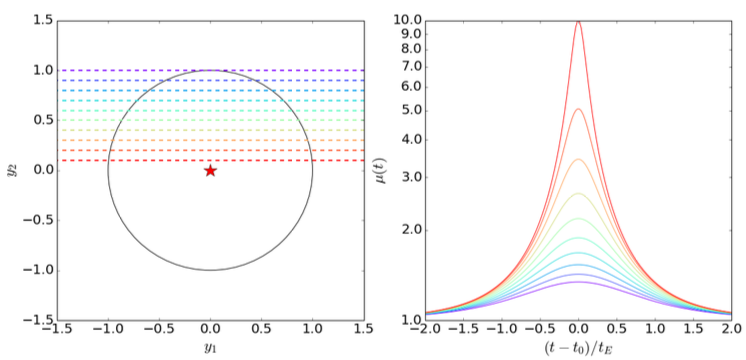
\includegraphics[width=\linewidth, keepaspectratio]{img//chapter3/light_curves.png}
    \caption[Microlensing light-curves for different impact parameters]{Left panel: some examples of source trajectory across the Einstein ring with different impact parameters $y_0$. Right panel: corresponding light-curves.\\\small{Credits: \cite{meneghetti_introduction_2021}.}}
    \label{fig:light_curves}
\end{figure}

The \emph{standard} microlensing light-curve of a simple point-source, point-lens system is thus described by four parameters: unlensed flux $F_s$, $t_0$, $y_0$ and $t_E$. Of these, $F_s$ can be measured in the absence of microlensing, $t_0$ and $y_0$ from the position and height of the light-curve peak, respectively. Only $t_E= D_L \t_E / v$ contains physical information about the lens system and determines the peak width, \ie the duration of the event. Assuming that the source distance can be determined from its properties (membership in a stellar system, spectral type and apparent magnitude), there are three physical parameters, lens mass $M$, lens distance $D_L$, and lens relative transverse velocity $v$, to determine from one observable: this is the so-called \emph{microlensing degeneracy}. 
Although the standard light-curve model is successful in numerous instances, there exist circumstances where some foundational assumptions of this model no longer hold. In such situations, it might be feasible to derive additional constraints that can partially lift the degeneracy. Non-standard light-curves, for instance, may occur when either the source or the lens are not point-like, or when the path of the source moving relative to the lens is not linear. Such instances often occur when either the lens or the source, or both, are part of binary systems.